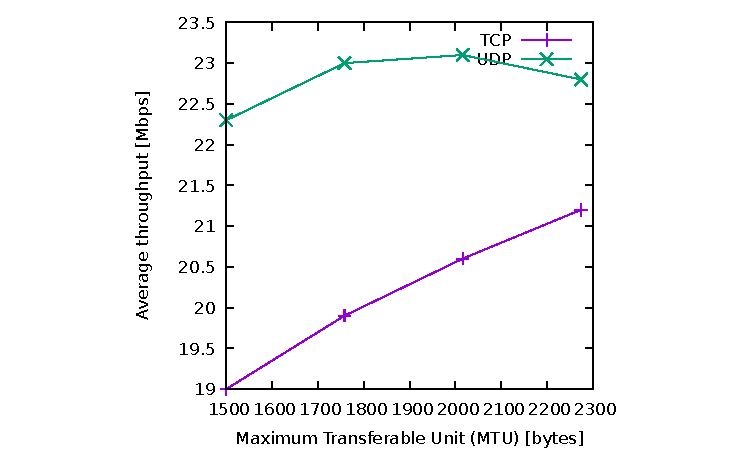
\includegraphics[width=0.5\textwidth]{traces/L3-4-1-tput.pdf} \\
Increasing the MTU and thus the size of the packets leads to increasing throughput for both UDP and TCP. Every bump in MTU leads to a throughput increase of 1.7 to 2 Mbps. This can partially be explained by the fact that Iperf reports the throughput looking only at the application data. Header sizes are 32bytes for 802.11, 40bytes for IPv6, 8bytes for UDP and 20bytes for TCP, leading to a per-packet overhead of 80 and 92 bytes per packet for UDP and TCP respectively. The larger the packet size, the lower the relative overhead of the headers. In a sense, iperf subtracts the header overhead from the actual packet throughput by only reporting the application data throughput.
\\ \\ This alone is not enough to explain the increase in throughput though. Let's consider UDP for the first two MTUs. At 1452 bytes per packet, the headers are ~5.51\% of the application data in size. At 1710 bytes per packet this drops to ~4.68\%. If we consider the throughput regarding the entire packet, the throughputs rise to 30.9 and 32.7 Mbps respectively. The relative gap between them is only slightly smaller than before, and thus still largely unexplained. Another interesting observation is that for UDP each increase in MTU decreases the reported packet loss by roughly 4\%. By looking at a trace of the tests, it is clear that (almost) all packet loss occurs before the packets are actually sent, as opposed to in the air or at the receiver. This seems to indicate the packets are dropped deliberately at send queues. A detailed explanation of why the percentage of dropped packets is so significantly different depending on the MTU would require thorough knowledge of how the queues work (both at TCP/UDP and wnic level). Some quick Googling indicated more people have noticed this effect, but nobody was able to offer a detailed explanation for why it occurs. \\ \\
(While all other data was gathered during the same session, this exercise was performed at another time. This explains why throughputs in this graph are higher than in the others).
